\section{Introduction}
\label{sec:intro}
\subsection{Motivation}
\subsection{Setup}
\label{subsec:setup}
We formalize the above discussion as follows. Assume $\mathcal{X} \subseteq \R^n$ to be a given (known) subset in the data space, and consider a signal (or image) $\mb{x}^* \in \mathcal{X}$. We construct $\mathbf{A} = \left[\mathbf{a_1~a_2~...~a_m}\right]^T$ with i.i.d. Gaussian entries. We aim to recover the original signal $\mb{x^*}\in \R^n$ from its compressed modulo measurements $y_i$ defined as:
\begin{equation}
y_i=\mod(\langle \mathbf{a_i} \cdot \mathbf{x^*} \rangle,R)~\textnormal{for}~i = \{1,2,...,m\},
\label{eq:modmeas1}
\end{equation} 
where $\mod(\cdot)$ is modulo operation with respect to a fixed, real-valued parameter $R$. We set $m<n$. For simplicity, we assume that the modulo function operates only within two periods, one each on the either side of the origin, as shown in the Fig.~\ref{fig:modop}. The primary assumption in our model is that the natural signal $\mathbf{x^*}$ is $s-$sparse in a chosen basis. 

\begin{figure}[h]
	\begin{center}
		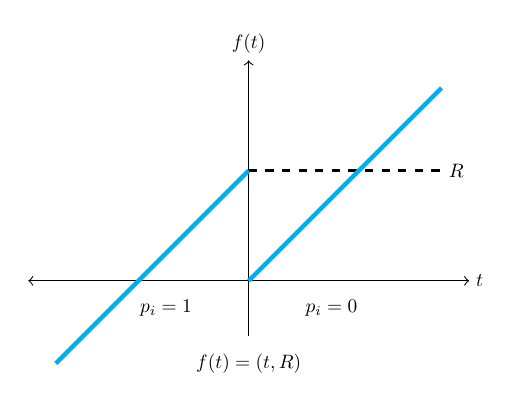
\begin{tikzpicture}[scale=0.7, every node/.style={scale=0.7}]
		\draw[<->] (-4,0) -- (4,0) node[right] {$t$};
		\draw[->] (0,-1) -- (0,4) node[above] {$f(t)$};
		\draw[scale=0.5, dashed, thick] (0,4)--(7,4) node[right]{$R$};
		\draw (1.5,-0.5) node(below) {$p_i = 0$};
		\draw (-1.5,-0.5) node(below) {$p_i = 1$};
		\draw (0,-1.5) node(right) {$f(t) = \mod(t,R)$};
		\draw[scale=0.5,domain=-7:0,smooth,variable=\x,cyan, ultra thick] plot ({\x},{\x+4});
		\draw[scale=0.5,domain=0:7,smooth,variable=\x,cyan, ultra thick]  plot ({\x},{\x});
		\end{tikzpicture}
	\end{center}
	\caption{\emph{Modified modulo function for the given problem}}
	\label{fig:modop}
\end{figure}

\subsection{Our contributions}
\subsection{Techniques}
\subsection{Paper organization}
The reminder of the paper is organized as follows. In section~\ref{sec:prior}, we briefly discuss the prior work. Sections~\ref{sec:prelim} contains notation and mathematical model used for our analysis. In section~\ref{sec:algo}, we introduce the MoRAM algorithm, and provide a theoretical analysis of its performance. We demonstrate the performance of our algorithm by providing series of numerical experiments in section~\ref{sec:exp}. Section~\ref{sec:disc} provides concluding remarks.